\documentclass[10pt,twocolumn]{article} 

% required packages for Oxy Comps style
\usepackage{oxycomps} % the main oxycomps style file
\usepackage{times} % use Times as the default font
\usepackage[style=numeric,sorting=nyt]{biblatex} % format the bibliography nicely

\usepackage{amsfonts} % provides many math symbols/fonts
\usepackage{listings} % provides the lstlisting environment
\usepackage{amssymb} % provides many math symbols/fonts
\usepackage{graphicx} % allows insertion of grpahics
\usepackage{hyperref} % creates links within the page and to URLs
\usepackage{url} % formats URLs properly
\usepackage{verbatim} % provides the comment environment
\usepackage{xpatch} % used to patch \textcite

\bibliography{references}
\DeclareNameAlias{default}{last-first}

\xpatchbibmacro{textcite}
  {\printnames{labelname}}
  {\printnames{labelname} (\printfield{year})}
  {}
  {}

\pdfinfo{
    /Title (A Cocinar: Experiencing Mexican Culture through cuisine in VR)
    /Author (Stephanie Enriquez Isais)
}

\title{A Cocinar: \\ Experiencing Mexican Culture through cuisine in VR}

\author{Stephanie Enriquez Isais}
\affiliation{Occidental College}
\email{senriquezisa@oxy.edu}

\begin{document}

\maketitle

\section{Introduction}
“A Cocinar” is a virtual reality game in which players learn more about Mexican cuisine through cooking Mexican dishes. They play from the perspective of a Mexican American character learning to cook by being instructed through messages from their Mexican parents. The aim is to give users a new and open perspective on Mexican culture and cuisine. 

\section{Problem Context}
Mexican cuisine is extremely diverse and has a lot of cultural significance. There are drinks, like tepache (fermented pineapple juice), that have pre-colonial roots and are still widely enjoyed by people in Mexico. However, unless you live in Mexico or have some Mexican heritage you probably won’t ever encounter these parts of Mexican culture in the United States. Therefore, Americans base their beliefs of Mexican culture on stereotypes presented to them by fast food chains who benefit from commodifying cultural cuisine, like Mexican cuisine, as authentic so they can sell more. As Taylor Griggs writes in “Globalization, Glocalization and the Symbolic Economy of the Taco”, “it is easy to distribute commodified Mexican cuisine across the global market because it acts as a safe, working, and economically successful representation of Mexican culture- despite the fact that its culture signifiers, now commodified, commercialized, and removed from their native context, are devoid of their original cultural meaning and articulation” \cite{tacoEcon2017}. The problem lies in the fact that this commodification and commercialization takes away the cultural meaning and benefits from propagating stereotypes about Mexican culture. Jefferey Pilcher, in his book “Planet Taco”, notes that as Mexican cuisine began to gain global popularity, many restaurants chose to “reproduce a stereotyped hacienda theme with images of cacti, sleeping peons, and china poblanas in low-cut peasant dresses” \cite{planetTaco2012}. This means that over time, unless we make a conscious effort to remember and value the original cultural meaning of Mexican cuisine, it will continue to deviate from its original form to form something that is a “credible approximation of Mexican regional cuisine” \cite{planetTaco2012}. This desire for authentic Mexican food that fits into the Americanized version of authenticity is something Alexandra Ibarra discusses in her thesis “ "Eating Real Mexican: Identity, Authenticity, Americanization, Health, and Food Culture in the United States After 1900" \cite{realMex2022}. She writes, “it was a safe type of “authenticity” however that had to toe the line of being ethnic enough to be considered adventurous and cosmopolitan, but never too ethnic” \cite{realMex2022}. It is clear how the commodification and commercialization of Mexican cuisine in the United states drives this “safe type of authenticity” in Mexican cuisine that limits the true cultural significance from being expressed. This creates a cycle of continuously changing Mexican cuisine to what is “authentic” so it can sell and because it sells it is considered “authentic. Therefore, my game “A Cocinar” aims to expose players to that Mexican culture that is not prevalent in the United States by having them cook Mexican food in VR; taking advantage of the strength VR has in storytelling and immersion to get them to learn about Mexican culture. The goal is that it provides players with a new and more open idea of what Mexican culture is even if it comes from the limited scope of the Mexican American perspective.
 
 

\section{Technical Background}
\subsection{Unity Game Engine}
“A Cocinar” was created using Unity and their XR interaction toolkit \cite{xrUnity2022}. This is a component based interaction system for creating cross platform VR and AR experiences. It provides the locomotion, selection interaction and UI components needed to start building a VR game. An important part in understanding how VR game development works in Unity is their 3D object setup. Every 3D object in Unity is made of a mesh which stores the object's vertex data and gives it its visual form \cite{meshUnity2022}. If you want to detect when an object has interacted with other objects or just give it size in the physical world you need to add a collider. Colliders achieve this by “define(ing) the shape of an object for the purposes of physical collisions”\cite{colliderUnity2022}. In addition there are hierarchies between the different types of colliders. There are 3 types of colliders, Compound or primitive colliders, mesh colliders and static colliders. Compound or primitive colliders are basic 3D shapes like a box, sphere or capsule that approximate the shape of an object while keeping a low processor overheard\cite{introCollisionUnity2022}. Static colliders are used for things like floors which need to have a physical shape in the world but will not be dynamically moved around. Mesh colliders are differentiated from the others because when they are in convex form, they mold themselves to an object which helps make it interact with objects in a manner that best fits the shape of their assigned object. However, this accuracy comes at a cost, the Unity Manual recommends using a combination of primitive colliders, to roughly give shape to an object, over the use of a mesh collider because they are more expensive performance wise\cite{physicsUnity2022}. This recommendation is an example of how Unity is not geared towards a very detail oriented physics based game, like “A Cocinar”, because while this rough estimation with colliders might work for a gun that will only be held in one position, a fruit that will be held and moved around by the user needs to have more accurately sized colliders. Finally, there are rigidbodies which give the 3D objects their physics. This includes things like gravity, mass, drag and other types of physic based properties \cite{rigidBodyUnity2022}. In summary adding a 3D object like an apple to a Unity game requires making the mesh, adding a properly sized collider and then setting up the physics logic for how it interacts with other objects. While this may sound simple, as you will learn later on it is not meant for the level of detail needed to create a game that has a cooking simulator component.


\section{Prior Work}
\subsection{Cooking Games}
When doing research into the prior work done to address this problem, I found a couple of VR apps that are related or inspired me when building “A Cocinar”. The first one is called Lost Recipes\cite{lostrecipes2022}, this VR game teaches users to cook by showing an array of traditional dishes from ancient cultures like the Mayan, Greek and Chinese. The game guides the players through tasks like measuring and mixing ingredients in an effort to recreate a traditional recipe. While this game does a good job of encouraging the users to complete the tasks and even try the recipes out on their own (this is based on some reviews left on the game), it doesn’t give much information about its significance a food item or a technique has to the people doing them. Since this is the game that is most similar to my idea, it has helped me identify the areas that I would like to improve on. At the same time, playing the game has taught me about the manner in which affordances can be used to have the user complete the game in the intended manner and gain the most out of it. Another similar cooking game is Cooking Simulator\cite{cookingsim2019}. As the name suggests this game is a lot more focused on creating a realistic experience of what it is like to cook in VR. The user can to measure each ingredient, cut the produce and even cook or bake in the game. This game is probably one of the most realistic cooking simulators and gives good examples of how to program the tools in the kitchen so the user can use them with controllers. When looking at references for how to build my cooking mechanics this game gave me inspiration for how I would like things to work. 

\subsection{Storytelling Games}
In addition to the cooking aspect of my project, I want to really take advantage of the immersiveness of VR and create a VR experience that can tell a story in a more engaging way. The first example is the VR game “Vader Immortal”\cite{vadarimmortal2019ep1}. The game revolves around the player trying to stop Darth Vader from completely destroying the planet Mustafar. When presenting the player with the history of the planet and why they should fight for it, they do it through the use of 3D animations. The majority of the game is the user traveling, fighting, and exploring the world but when presenting what is at stake, the creators decided to use storytelling through animation and after playing the game, it is clear why they made this choice. Seeing the story quite literally unravel around you makes it more engaging and immersive. It inspired me to create a similar sentiment by presenting the player with personal anecdotes of the player’s parents in an effort to show them why what they are doing matters. Another technique for storytelling that inspired me was that of the VR game “What Remains of Edith Finch”\cite{finch2019}. This game details the stories about what happened to the Finch family and one scene does this very interesting of incorporating the mundane chore of cutting fish heads in an assembly line with character’s daydreams slowly taking up more and more of the screen space. This technique of using the mundane tasks as an opportunity to have the player see or hear more about the story is something that inspired me to add oral anecdotal stories when the player is cutting or cooking. This helped me add more of that cultural significance to the game and make mundane tasks like cutting more interesting.

\section{Methods}
\subsection{Development Process}
The development process for this game was similar to that of any other VR game. I began by doing research on the recipes that I wanted to include and created a storyline while noting what cooking mechanics would be necessary. I then started to create and implement those mechanics with rough models. Once I was at a good place with the cooking mechanics I bought or made my own 3D models of the ingredients and added them into the scene. It’s interesting that because some of the ingredients like the nopales or piloncillo, which are not common in American cuisine, I couldn’t find any suitable models of them so I made my own. Once the final kitchen and food models were implemented I had to create the recipe system that would let the user know when they have completed a step of the recipe and show them the next step.\par
While the general development process seems straightforward there was a lot of informal user testing with other people to fine tune the details of the game. I will talk more about the influence it had in the following sections. I will focus more on the unique decisions I had to make for my game and how I worked around the limitations of Unity. It is important to note that during my development process I had a major turning point in my game where I changed the focus of my game from portraying that of the general Mexican experience to that of the Mexican American perspective, heavily influenced by my own experience. As I will talk more about in the ethical considerations sections this is done to address the bias and overgeneralization that comes from making a game trying to portray a whole culture. 

\subsection{Locomotion}
Movement is a major component in every VR game because it allows users to traverse large virtual spaces while staying within their limited physical space. In VR there are 2 main ways of locomotion, teleportation and continuous movement \cite{teleportVRs2021}. As the name implies, with teleportation, the user is able to move around the space by using their controller to raycast a spot they want to appear in and then be teleported to that spot. One of the biggest advantages this locomotion method has it is considered the safe locomotion type in VR because it “doesn’t generate any optical flow, and thus reduces the risk of vection induced VR sickness” \cite{teleportOF2018}. Continuous movement allows the user to move around by using the joystick on their controller to hover around the virtual space, most closely resembling walking. However, this can cause users motion sickness because it does generate optical flow which is the “the pattern of apparent motion of objects, surfaces and edges caused by relative motion between an observer and the visual scene”\cite{teleportOF2018}. This apparent movement between the observer and their environment can cause vection, the perception of self motion without actually physically moving, which is more likely to create motion sickness. \par
For “A Cocinar”, I decided to use continuous movement because I wanted my game to simulate reality as much as possible and teleportation is not possible in the real world. When testing teleportation I also found that the short time everything went dark, it felt like I was being taken out of the game and it broke the sense of immersion. In addition, as noted in the article “Combating Vr Sickness: Debunking Myths and Learning What Really Works”, acceleration can increase motion sickness when continuously moving in VR and I constrained the speed to one level in my VR game\cite{vrSickness2018}. I was able to determine a comfortable speed by doing some informal user testing in which users gave me their feedback on how they felt after moving around at different speeds for a couple of minutes.  \par
To further combat motion sickness, I decided to implement a vignetting effect when the user moved around. It is also commonly used in other VR games to help reduce eyestrain and motion sickness. However, if it is not implemented correctly, it can actually increase motion sickness in users \cite{vignette2018}. Therefore, when adding this function to “A Cocinar” I did some informal user testing in which I presented different vignetting intensities to find what worked best for users.

\subsection{Cooking Mechanics}
The cooking mechanics were one of the most important parts of the game because it involved the main action users had to do. For this version of “A Cocinar” I implemented 4 cooking mechanics: cutting, dethorning, cooking and scooping. This is where I had to make some important decisions on how realistic vs functional I should make each mechanic. As briefly mentioned in the Technical Background and you will soon learn more about, this comes from the limitations of Unity’s physics system. The reality is that Unity is a game engine made to create all types of games but mostly shooters or other types that loosely mimic reality. While that can cause some comedic value by having objects jump or move in ways that they would never in real life, that was not the intent of my game. Therefore, a lot of the decisions I had to make on making mechanics more functional came from reducing the level of realism so that it didn’t as heavily rely on the physics system of Unity.

\subsubsection{Cutting}
The cutting mechanic was the first one I tackled and where I was first introduced to this problem. I originally wanted to make a knife that would cut a food item at any angle that it collided with the item. This means that it would have to cut through the mesh of the 3D object. Although there are Unity packages that can cut through a mesh there are several problems that arise. The first is that these tools can cut an object's mesh but one of the two cut halves will disappear. The second, and most important, one is that the tools can cut a mesh but not the collider of an object. As mentioned in the Technical Background, colliders are what allows objects to be picked up by the user and create scriptable events when colliding with other objects. Therefore, having a collider that correctly fits the mesh of an object is essential to creating the illusion that you are holding a piece of that object. However, as you can see in figure 1, the image on the left shows the original cube and this has a box collider on it, however, the image on the right shows a piece of that box that has been cut out but it is floating. This is because the original box collider is still on that piece when in reality it needs a much smaller collider. This creates a problem in that the object would still interact with others as if it’s the original bigger box not the smaller piece. I then realized I could not go with the realistic version of cutting in my game and I had to come up with a more functional mechanic that would still give the illusion of cutting. Therefore, I decided to pre-cut 3D models and add a script to each piece that would detect a collision between a cuttable food item and a knife, destroy the uncut piece and instantiate 2 new smaller cut pieces. In this way I could add the proper size collider to each piece before it was instantiated.\par

\begin{figure}[h]
\caption{Example of mesh cutting}
\centering
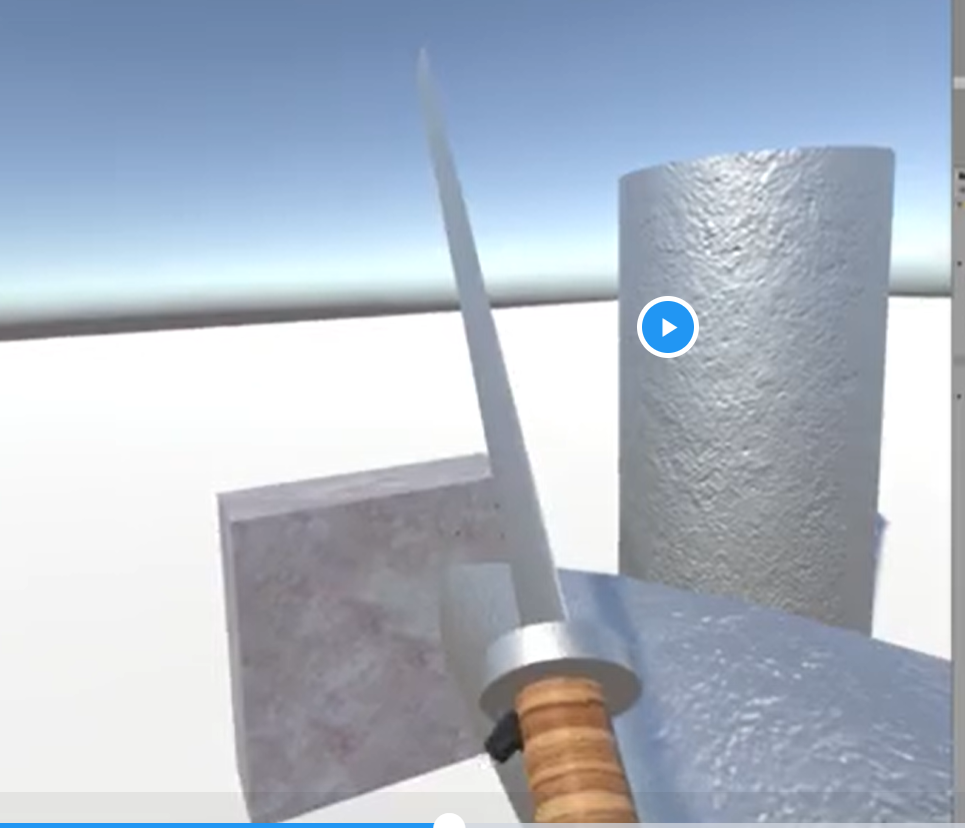
\includegraphics[scale=.2]{Screenshot_20221214_105111.png} \cite{meshCut2022}
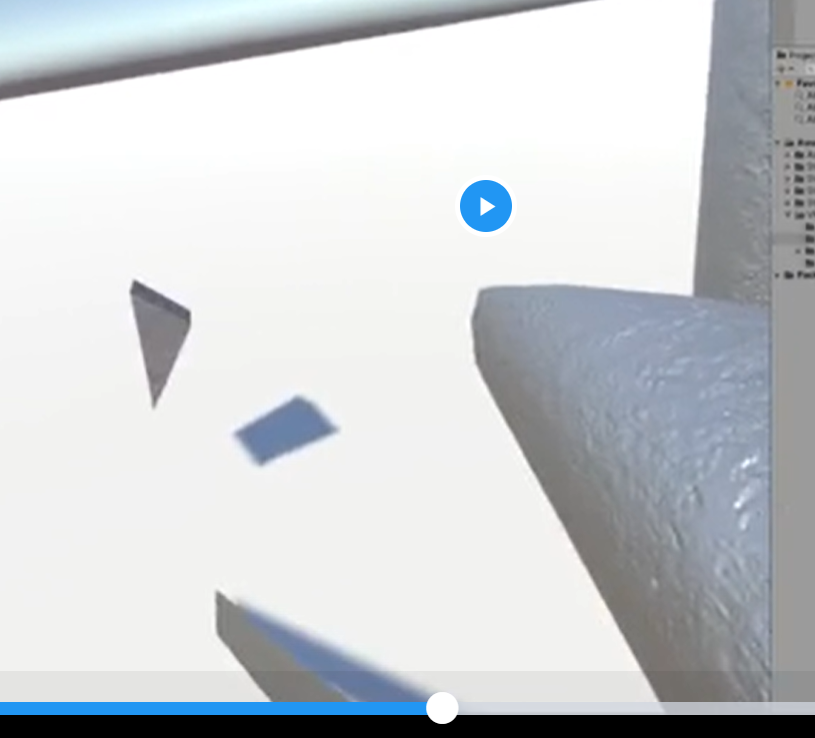
\includegraphics[scale=.2]{Screenshot_20221214_105133.png} \cite{meshCut2022}
\end{figure}

I did some user testing with this feature and I found that while it did cut the larger objects into smaller pieces there were 2 major issues. The first was that when a user touched the full cuttable object, it would trigger collision on that layer and all the pre-cut versions until it got to the smallest cut version in one swing of the knife. The second issue was that while the knife was touching the food item, it would keep creating new instantiated versions of the next level of that pre-cut item. Therefore, a tomato that is meant to cut down to 16 versions of one pre-cut 1/16 of the tomato, would have dozens of 1/16 parts of a tomato. This didn’t make logical sense because when you cut a food item, it doesn’t grow in quantity. After finding this through user testing, I fixed it by making the knife wait until the end of each frame before allowing the knife to cut so that gave users the time to move their knife and make one cut at a time that produced the 2 smaller pre-cut versions of that item. 

\subsubsection{Dethorning}
On the other hand there were cooking mechanics that I took the extra time to make as realistic as possible because I thought they provided important cultural knowledge about the amount and type of labor that goes into making a Mexican dish that can only be learned from doing it. Therefore, when it came to preparing the nopales I knew that most people had not eaten one, much less prepared one so I wanted to give them a more realistic experience. This involves taking a knife and scraping each of the thorns off of the nopal. I created this dethorning mechanic by turning off physics for a thorn while it was on the nopal and once it was hit by a knife it would turn it’s physics back on and fall off.  While I could have just told the user that their parent had already cleaned the thorns off I knew that the thorns on a nopal are a defining factor. In addition, it provided an opportunity to build the story by having the parent tell an anecdote about their experience doing that as a child in Mexico. When testing this with users I was pleasantly surprised to see how such a simple action seemed novel and interesting to them.  

\subsubsection{Scooping}
While creating the cooking mechanics and deciding how realistic to make each I decided to reference back to Lost Recipes and see how they implemented some of these features. I found that they definitely sided with being more functional and less realistic. I wanted to put more realism in my game but it still gave me ideas on how to make simple cooking mechanics like the scooping of spices. This is a very common action that most people do so I decided this would be a appropriate place to go with the more simplistic version of scooping in which the user put a spoon in the spice and it simply appeared on their spoon as a mass; rather than having each grain be picked up by the spoon. This also helped me lower my performance overhead because as I mentioned in the technical background, colliders should be used only when necessary and having a thousand or more of them as the grains of salt needed for a teaspoon seems unnecessary \cite{introCollisionUnity2022}. The aspect of this mechanic that was refined using user testing was the angle at which a spoon should “release” the spice and have it disappear from the spoon.\par 

In addition to that, I ran into a issue with the mesh colliders in Unity. Although they are supposed to mold to a object, they do this in a convex manner not concave. As you can see in figure 2, a convex collider doesn't mold well onto objects with space in between. This became a problem for things like using a bowl because it didn't allow for anything to go inside. I was able to solve this by buy a add-on called Technie Collider Creator 2\cite{techie2022}, this generated better fitting concave colliders by making them out of a bunch of primitive colliders. Again, as you can see in figure 2 it made the colliders fit a lot more snug and allow for scooping things out of a bowl. \par
\begin{figure}[h]
\caption{Example of colliders}
\centering
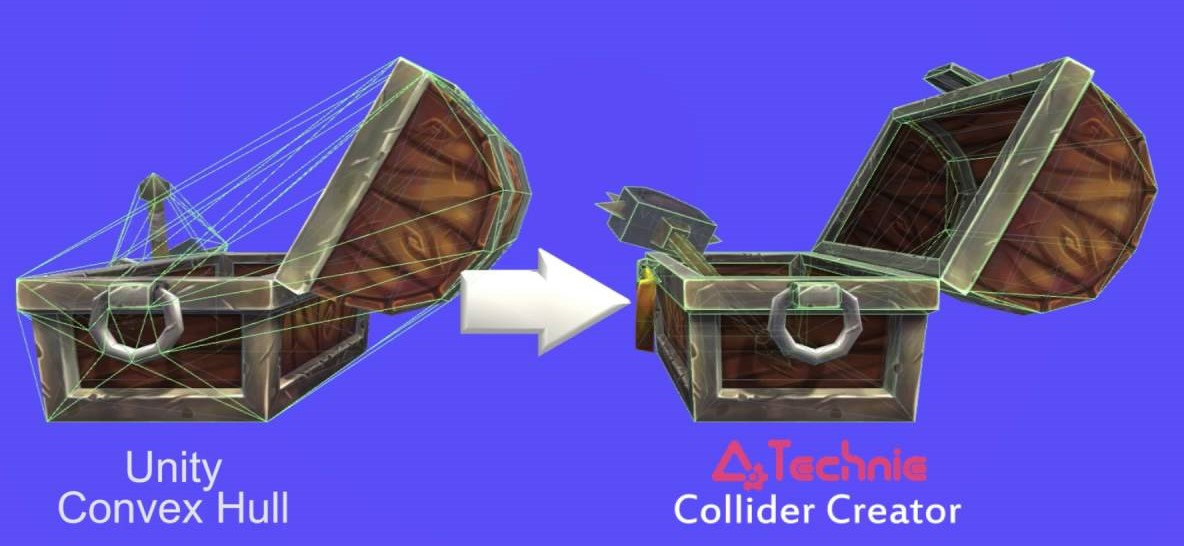
\includegraphics[scale=.2]{collider.jpg} \cite{techie2022}
\end{figure}


\subsubsection{Cooking}
Although the level of realism a mechanic should have played a large role in my design thinking as I created these cooking mechanics there were times when it didn’t matter as much as taking the time to build a well structured recipe system. For my game a recipe system is what I call the scripts that listens for when a step of the recipe is done and continues to the next. This is similar to a Game Controller or Game Manager scripts often used in game development but it functions on the level of one specific recipe not the whole game\cite{gameManager2021}. At first I implemented cooking as something simple in which a cookable object waits for it to collide with a pan and then it starts the sizzling sound effect as well as the color changing of the object to show it’s been cooked. However, when doing user testing on this mechanic I found that sometimes users would pour the cookable items on the pan before they set it on the stove and so the sizzling and cooking would start without any heat. This didn’t make any logical sense as a cooking mechanic but I realized that I hadn’t caught this because I had always placed the pan on the stove first so I hadn’t thought to add a script to make sure the pan was on the stove before the cooking began. This taught me the value of having other players test my game because I cannot assume that the user would play the game the same as I did. Moving forward with this game I will make sure to add more of these check marks in the recipe system. 

\subsection{User Interface (UI)}
The UI elements of A Cocinar were very important because that was the main way the character’s parent would interact with the user and tell them the next steps of the recipe and provide the cultural knowledge. In addition, implementing a Heads Up Display (HUD) is essential to creating a game in which the user can have control over the game settings like pausing and sound.  

\subsubsection{World Space Tablet}
The player receives information about what steps to take from a world space UI in the form of a tablet that receives messages from their parents. Originally the instructions would just be received in the form of audio messages that the user would play from a wrist menu. However, I realized that it was unclear how that fit into the world and storyline. Therefore, I decided to make the messaging system more clear through the use of a world space tablet that can be moved around as desired. I designed the interface to look like the iMessage and Messenger interfaces so the user would be able to recognize what the tablet was displaying. When it came to how the user would select buttons on the tablet I had the choice of using a direct touch or raycasting interaction technique \cite{learnXR2020}. Both of these are very commonly used in VR and at first I wanted to have a direct touch interaction. However, because I decided to make the hands spheres (since including hands required a lot of work in fine tuning the physics when interacting with other objects) I couldn’t use the direct touch since there would be no pointer finger to select a button on the screen. Therefore, I went with raycasting and although it works well for selecting small things on the tablet screen, user testing showed that the raycast would sometimes be triggered even if the user didn’t mean to interact with the tablet. I attempted to fix this by having the raycast only work on UI elements but I found that if the tablet was in the range of the raycast, it would sometimes grab the tablet. Moving forward, I will take the time to properly implement hands in VR so the user can directly interact with the tablet.
 

\subsubsection{HUD Wrist Menu}
While it makes sense to have the messaging system in the form of a tablet be a part of the world as it is a part of the storyline, the UI for the settings did not fit that same role. This was something that needed to be more of a HUD for the user to quickly access and change settings. When doing research into the HUDs I found that there are two different types, the first is called a diegetic HUD which means it stays mounted to the user's view and moves as the user moves \cite{HUDS2020}. The second is a non-diegetic HUD and this one does not move with the user’s head movement but is tied to some other part of their body or outside of it as well. Although diegetic HUDs are more commonly used in traditional screen based games, research about “The Effects of Different Types of HUDs on Cybersickness” shows that, in VR, they can actually cause more motion sickness than a non-diegetic HUD \cite{HUDS2020}. Therefore, I decided to include my setting UI in the form of a dynamic (can be open and closed) non-diegetic HUD on the user's wrist. This type of HUD system is also something that I have seen in other continuous movement VR games like Green Hell and Star Wars: The Galaxy’s Edge \cite{talesOfGlax2020}. During user testing, users seems to like using the wrist menu since it reminded them of a apple watch. 

\subsection{Audio}
The visuals and audio in VR go hand in hand in creating an immersive experience therefore I tried to be as meaningful as possible in the type of audio I added to “A Cocinar”.

\subsubsection{Sound Effects}
For the sound effects of my game I decided to part with my friend and Music major Alana Duvall to create custom sounds for my cooking mechanics. Sound effects in all forms of media, whether it’s movies, games or VR experiences are essential to immersing the users in the world being presented. A study on the effects of sound effects in games showed that when comparing a game that didn’t have sound effects to one that did, most users felt more immersed in the game that included sound effects \cite{audioIm2013}. Since I wanted to create a realistic experience when cooking, I decided to get help with creating custom sound effects because for things like dethroning a nopal, I could not find something that gave that audio effect online. When doing user testing, it was interesting to see how immediately users made note of the sizzling and how that added to their level of immersion in the game.


\subsubsection{Voice Over}
Part of learning to cook family recipes from Mexican parents who got their recipes from their parents is that there isn’t always a written recipe with measurements. It often involves being told to put a pinch of this or a handful of that. I wanted to recreate that experience by hearing the voice of the player’s parent tell them the instructions in conjunction with the written message. Since I added this feature in the middle of user testing, I was able to clearly see how much of an influence it has on the user’s playthrough. For the users that had the audio playing to them, they would ask me less questions on what the next step was or how to do something. Currently the voice reading the messages is my own but moving forward I would like to have my mom record it. I think that having a real mom tell the user the instructions will allow the users to better immerse themselves in their character. 

\subsubsection{Background Music}
Research shows that background music is essential to helping immerse players in the game. A study on “The Influence of Background Music of Video Games on Immersion” \cite{backA2015}, showed that the background music can help create a sense of physical space in 2D games and this is only further emphasized in VR games because you can have 3D spatial audio that helps build the illusion that you are in a real room cooking away. In addition to that, including background music is essential to the Mexican cooking experience because similarly to how you learn about cooking or life through what your parents tell you, you learn about music through what your parents play for you. There is a sense of nostalgia that comes from listening to older Mexican music and remembering the time your parents would play it when you had to do some sort of chore. I wanted to give players that same experience so that if they ever heard those songs again they would remember the game and the cooking they did. When choosing the songs for this game, I went with older songs that people of one or two generations ago would consider their generation’s music. While testing the game I found that most users would make a comment about the music playing and how it made them feel more in the zone. 

\subsection{Content}
As I mentioned in the introduction, the purpose of this game is to provide a new perspective on Mexican cuisine. Therefore the content that I included was very important to consider. Since my initial approach was to give people a look into Mexican cuisine as a whole I found that it was hard to find a recipe that could take on such a big task when Mexican cuisine varies so much from state to state. Therefore, approaching this game from the Mexican American perspective helped me narrow it down to something that was easier to handle because it was more honest in its limitations as a view into Mexican culture.

\subsubsection{Recipes}
When it came to choosing the recipes I had 3 requirements. One that it was something my parents had taught me and was common in their respective families. This helped me choose recipes that are relevant and actually eaten by people. Second, that it had something authentically Mexican about it. This was a bit more nuanced but I determined this by choosing recipes whose main ingredient or recipe were present in indigenous Mexicans diet before the Spanish conquest. Third, that it was a healthier dish not commonly seen in the United States. This was to directly combat the stereotype that Mexican food is unhealthy and bring some novelty to the player.  \par
Currently the two recipes included, the first is a nopal salad whose recipe I got from my mother. The nopal is a staple vegetable in Mexican cuisine and is so significant to our culture that it’s even on the Mexican flag. Nopales have been eaten by Mexican people since the pre-hispanic days and continue to be consumed today \cite{cacti2002}. The second recipe included in “A Cocinar'' is a fermented pineapple drink called tepache. This drink has pre colonial roots and was originally used by Mayans as a sacred drink \cite{tepache2021}. I got this recipe from my father and what's so interesting about tepache is that there is no one master recipe but it varies from person to person with some adding additional fruits or spices. 


\subsubsection{Script}
The first iteration of my script was simple in that it mostly provided instructions on how to make each recipe and some general information about the benefits of the ingredients like the nopales helping with diabetes. However, as I will discuss in my results sections, after user testing, I found that my original script was lacking in immersing the players in their character. Therefore, I have edited the script to include more anecdotal stories from the player’s game parent about their experience with making each recipe in the past. I think this will make the storytelling stronger because it brings more of a human touch to the game and will remind users of hearing stories from their own parents.

\section{Evaluation Metrics}
\subsection{Informal User Testing}
There were two main aspects of the game on which I wanted to evaluate how it performed. The first one was the VR experience and the second was the Cultural Immersion. As you may have noticed in the Methods sections, I did a lot of user testing when developing the different aspects of the game because of the iterative nature of game development. In my case this looked like asking a friend or classmate to test a specific mechanic while I watched them play, had them think out loud, took note of things that needed to be changed and implemented their feedback of the game. I had them think out loud as they were playing because the think-aloud protocol is a technique to help researchers understand a user's state of mind as they are experiencing the product \cite{testQues2021}. Watching the user as they test your product is also a common aspect of usability tests and I found that it provided me with details the user wouldn't think to tell me \cite{testing1012019}. For example, going back to the pan playing the sizzle sound before it touched the stove, this is something that I didn’t catch when I played the game but I immediately noticed when someone else tested it. Overall, this informal user testing helped me to fine tune the details of the game mechanics but I saved the full playthrough user testing for my formal user testing session.

\subsection{Formal User Testing}
Once I felt like the game was in an appropriate state to test, I recruited 5 people to formally test my game. I choose 5 because as Jakob Nielsen writes in an article about the ideal number of user testers, “elaborate usability tests are a waste of resources”\cite{5tester2000}. This was especially true in my case because the game play plus the interview would easily take more than 30 minutes. This time starts to add up and becomes less worthwhile because after a couple of people you start to see trends in the same things that need to be fixed. Going back to my two main focuses for the user testing, I decided to first have the player’s play the game and then interview them on their experience with playing in VR and with the cultural immersion of the game. \par
I originally set up the user testing to have each person take a survey before and after playing the game to determine if they had learned something about Mexican culture through the game, however, after doing some research on how to write questions for user testing I realized that I needed to interview users instead of just having them answer surveys. This was because during my research on question writing I learned that asking open ended questions is important to receiving the kind of qualitative feedback I needed to properly evaluate what the users were getting out of the game \cite{testQues2021}. Surveys on the other hand provided quantitative information that wouldn’t give me the level of detail I needed to understand what a user got out of my game.

\subsubsection{VR Experience}
For the formal user testing on the VR experience, since I used informal user testing to fine tune the cooking mechanics, I didn't ask specific questions about each mechanic. However, I did want to evaluate, through the use of open ended questions, if the combination of all the mechanics made the user feel like they were cooking. This is because the cooking aspect is integral to the game and teaching the users about the cooking techniques used in Mexican cuisine. Another important aspect I wanted to evaluate was if my game caused less motion sickness in users than other VR experiences. As I will talk more about in the ethical considerations section, 40\% to 70\% of users experienced motion sickness in VR \cite{motionsicknessvr2019} and part of the interview asks users if they experienced motion sickness to see if the strategies I put into place to reduce motion sickness worked. The final aspect of my game I ask users about is their general feedback on what the user enjoyed playing in the game. At the end of the day, games are supposed to be fun and I want to evaluate what about this game is fun. Again, I could have asked this question in a survey but I didn’t think that a scale of how fun this game was would help me as much as qualitative feedback on what the users enjoyed. Since they could also tell me things like why they were fun or what could be done to make them better.

\subsubsection{Mexican Culture}
There were several aspects of what my game taught users about Mexican culture that I wanted to evaluate. The first pertains to the strength of the storytelling in the game. This is important because a lot of the cultural value comes from the anecdotal stories told by the parent. If the user isn’t immersed in that aspect then it means I have to better the script and storyline. The next aspect I want to evaluate is if “A Cocinar” had taught them something new about Mexican culture. This was because I wanted to make sure that there was some novelty and new value that “A Cocinar” brings to the players. If they said they didn’t learn anything that would mean that I could have possibly fallen into portraying the same stereotypes that are widely perceived about Mexican culture in the United states and this is not something I want to do. The last part I wanted to evaluate was if the game changed the player’s perspective on Mexican culture. I initially considered asking players what stereotype they believed about Mexican culture (to later see if they changed) but after doing intial tests asking people, I came to the conclusion that players did not feel comfortable showing that part of themselves. After going some research about this, I learned that it might be because people would not want to offend me by telling me outright what stereotypes they think about my culture. This is a common pitfall that is written about by the Interaction Design Foundation \cite{pitfall2022}. Therefore, I left the question open ended so that the players would tell me what they felt. 


\section{Results and Discussion}
For the informal user testing I did while building “A Cocinar”, the feedback I received was quickly implemented back into the game since the goal of that feedback was to help me build the mechanics of the game. One of the research tips that I learned about what to do with your usability testing results is to organize by priority so you know what is more important to fix first\cite{testResults}. This was especially helpful with the informal user testing because I was constantly iterating based on what I learned and that helped me prioritize be more efficient. Examples of this are further explained in the Methods section. However, for my formal user testing, I gained a better understanding of how (if at all) my game gave users a new and more open perspective of Mexican culture and the VR experience. To see the transcript of the interviews, see the “A Cocinar Interviews” PDF in this git repository.

\subsection{VR Experience}
Regarding the VR experience of “A Cocinar” I received very positive feedback. All of the users mentioned that they felt like they were cooking. When asked about their favorite part of the game, one user said “I liked how it was so hands on, every step I had a goal to it. The ding gave me serotonin, like yes I did that. I didn’t want it to stop.” The ding they are referring to was the completion sound that is played after a user completes a step and can move on to the next. The fact that all users felt like they were really cooking and like how each step had a goal to it was indicative that the cooking mechanics as a whole were well structured and well connected so that the user knew how one step led to the next. This helped me evaluate that my game did a good job at creating a sense of immersion in cooking and encouraging the user to keep playing and keep learning about Mexican cooking techniques. \par
When asked if they had experienced motion sickness while playing that game, 2 out of the 5 players said that they had. Although this is a small sample size, it does mean that 40\% of the participants in my user testing experienced motion sickness. When compared to the literature that says around 40\%-70\% of VR users experience motion sickness, my results are in the low range\cite{motionsicknessvr2019}. These results are not unexpected because, as I mentioned in the Methods, I knew that having continuous movement would create the possibility of more users experiencing motion sickness. However, by asking the users where they experienced motion sickness I now have a clear plan of where I can improve. As I mentioned in the evaluation Metrics sections, it was important to ask about motion sickness when playing the full game instead of just doing each mechanic because I actually found that users experience most of the motion sickness when walking around the kitchen, something that only needed to be done when playing the full game. \par
The final part of the VR experience that I evaluated was how fun “A Cocinar” was. This is where the time I put into making this an immersive experience came through. All of the users commented on how the fun came from how well tied together the game was. Almost all of the users mentioned that they liked the music playing in the background. One user commented that it made the kitchen “feel more homey and authentic”. While watching the users play the game I noticed that some would do little dances and others took the time to just explore the kitchen while they waited for something to cook. To me this showed the value in creating the right setting for the game.

\subsection{Cultural Immersion}
For the cultural immersion, I learned that my game was lacking in the storytelling aspect. Most of the feedback that I got during the interviews mentioned that users were not able to properly get into their character. In fact one interviewee said, “I didn’t really realize that I was playing as someone in specific, I thought I was just supposed to cook”. I think that clearly exemplifies how since I spent most of my time working on the cooking and game mechanics, the users were able to successfully play the game but they were not as immersed in their character as I thought they would be. Users mentioned that the idea of having the mom give instructions was good but that it wasn’t executed in a manner that made considering her as your own mother an integral part of the game. As I mentioned in the evaluation metrics, I added a question on the immersion into their character because I knew it would help me understand the quality of the storyline I wrote. Now I know that moving forward I will spend more time adding features that build a richer storytelling experience so that coming out of the game, they can gain a deeper understanding of Mexican culture by bettering getting into character. \par
However, while my game needs to improve in the storytelling aspect, when I asked users if they had learned something new about Mexican culture, all of them said they had. This was good to know because there was a wide range of cultural backgrounds from which the users came from. This also meant that I had done a good job at choosing recipes that provided some novel aspect to the user since not everything was new to every user. For the people that knew very little about Mexican culture, even the nopales as a food item was new to them. However, for the users who were Mexican or grew up around Mexican culture, their responses were different. One player, who is Mexican, when asked if they had learned something new said “I knew about the nopales being used in a salad but my family boils them instead of frying them”. This was very interesting to hear because it shows how Mexican cuisine is so diverse that even in the same dish there can be different styles of cooking it. More importantly, it shows that these types of experiences, that try to expand someone’s understanding of Mexican culture, can teach even a native Mexican person something new about their culture. \par
Finally, through the user interview I was able to evaluate how I had changed user’s perspectives on Mexican culture. I found that for the users who knew very little about Mexican culture, their perspective was more heavily influenced than those who were Mexican or had more exposure to Mexican culture. Users with limited previous exposure mentioned things like getting most of their exposure of Mexican cuisine from places like restaurants and that rather than changing their perspective, it added to it. On the other hand, users who knew more about Mexican culture said their perspective had not changed. One user said, “It didn’t change my perspective because I am familiar with aspects of it... I have a deep appreciation for the culture and I’ve been to Mexico so I know how what we see in the US is different from what it really is. It doesn’t even touch the surface”.  
\subsection{Moving Forward}
Overall, after this first round of official user testing, I learned alot about where my game could improve that even the informal user testing didn’t provide. I am not surprised that the game mechanics worked out better than the story immersion because I spent most of my time working on that. It is important to note that users still learned more about Mexican culture and in some cases it changed their perspective a bit. However, it could definitely be improved, which is what I will focus on in the next iterations of “A Cocinar”. Another strategy for how to analyze the results of usability test like these is to talk with you team \cite{testResults}. However, since I didn't have a team, I talked to other professors about what my results meant and how to fix them. For example, Prof. Aleem Hossain was a resource (after my first round of formal testing) for helping me build a plan of how I could improve the storytelling in my game. 



\section{Ethical Considerations}
While this game may be made with the best intentions in mind, it still has some ethical considerations to take into consideration. 
\subsection{Issues with VR}
\subsubsection{Motion Sickness}
One of the first ethical issues with this project is the medium in which it is played. As I mentioned in the technical background, motion sickness is a big concern for VR. In fact, 40\% to 70\% of VR users have experienced motion sickness after about 15 minutes of usage \cite{motionsicknessvr2019}. Even if I take all the necessary precautions to cause the least motion sickness there are still some factors out of my hand. Like the fact that women are more likely to get motion sickness in VR than men. An article about the issues of gender disparity in VR motion sickness states a possible reason for this imbalance to be, “gender differences in depth cue perception due to men favoring motion parallax (which is prioritized in VR) and women favoring shape-from-shading“\cite{vrbarriers2018}. As the article also later writes about, this inequity in design can also be due to designers favoring those who are ‘most likely” to buy and use VR equipment\cite{vrbarriers2018}. All of these explanations attribute the motion sickness gender imbalance to the inadequate design of VR headsets, something that as a creator of a VR project, I will not be able to change. 

\subsubsection{Accessibility}
Other factors that can exclude people from using VR are accessibility issues. An article by Wired discussed how people with physical or visual disabilities can have a harder time using VR. They mention accessibility consultant Erin Hawley, who has limited hand movement because of muscular dystrophy, could not use the Anne Frank VR experience because it required movements such as opening a door that she could not reach \cite{vraccessibility2022}. Some games, like Arca’s Path, try to address these issues in VR by implementing an option in which the user can control the ball with simple head movements instead of the controllers \cite{arcaspath2018}. While it is important to consider such matters, the reality is because of the limited time I had to work on this project, adding some of the accessibility approaches used by other games was not feasible. Therefore my project would not be accessible to everyone.


\subsection{Issues with Implicit Bias}
The most evident ethical concern lies in the implicit bias that can occur in the project creation process. Although I am Mexican and have grown up surrounded by Mexican culture I am in no way an all-knowing person when it comes to what is Mexican and what isn’t. Therefore, when creating the storyline for this project and assessing what should and shouldn’t be included, there is the risk of my implicit bias affecting the impression of what people learn about Mexican culture after using the experience. Implicit bias is an important ethical issue to consider because it is an unconscious way a person can be biased towards something. An article about the subject described how teachers can show bias toward students when it came to making a judgment call on disciplinary actions that have more subjective parameters, such as what it means to be ‘disrespectful’ or ‘disruptive’ \cite{implicitbias201516}. They found that the students of color were more likely to be disciplined because of the teachers’ experience and unconscious associations with race \cite{implicitbias201516}. This is relevant to my project because it shows that people's biases can come out when making decisions on subjective matters even if they are not consciously aware of it. This could be represented in things like the style of cooking I instructed users to do and even music I had them listen to. Which in the moment I just choose without thinking of how I was being biased towards a specific style or musical genre and how that would affect the overall perception of Mexican culture. While these are examples I can point out, the whole idea behind implicit bias is that I won't know I am being biased towards something but that bias will be passed onto my game and influence players' perspective of Mexican culture. 

\subsection{Overgenerization}
As I mentioned in my Methods sections, there was a turning point in my development process where I realized that I could easily run into the problem of overgeneralizing Mexican culture in the way I was framing my game. Which is ironic because that’s what I was trying to prevent other people from doing. As written in The Routledge Handbook of Language and Intercultural Communication, “overgeneralization is potentially problematic because there is always the risk, when trying to describe national cultural characteristics based on an inevitably relatively small scale survey, of overlooking the diversity that exists”\cite{overGen2020}. Mexican culture is very diverse and the reality of my project is that the limited time only allowed me to add 2 simple recipes. By previously presenting my game as an accurate representation of Mexican culture as a whole, whatever these 2 recipes and storyline show could overgeneralize the player's view of Mexican culture towards my biased view. Since Mexican culture is so diverse and I am only one person building this game I cannot guarantee there will be no bias. I can only try to be upfront about it and encourage people who are interested to learn more from other sources and gain a wider world view on Mexican culture. 

\subsection{Mexican American Perspective}
Therefore my approach to getting people to not overgeneralize Mexican culture was to emphasize that this game is from the Mexican American perspective, acknowledge the bias that exists in the game and make sure users know based on one perspective. By the Mexican American perspective I mean that similarly to how the players are experiencing this game through a second hand retelling, as Mexican Americans we often did not grow up in Mexico. The knowledge I have of Mexican culture is secondhand and heavily influenced and biased by my parents. The knowledge the players are receiving is forthrightly biased as well; from the perspective of their parent who is my character and written by me. In a way, this game channels the Mexican American experience of learning about a culture through the biased lens of our parents and what they are. We trust that their recipes and stories are true and believe them to be the right way. In that same way the players are trusting me and believing that what I show them in the game is a good representation of Mexican culture. 

%\section{Conclusion}


\printbibliography 

\end{document}
